\section*{Problem 3}
We have used in this problem a similar architecture for the VAE's decoder and the GAN's generator which is an MLP with 6 layers, as shown in this code snippet:
\lstinputlisting[language=Python]{gangen.py}

We have decided to go with this architecture, after having tested several architectures for both models, including convolutionnal neural network. We noticed that the VAE model works fine with a convolutional architecture whereas the GAN have not got good result with that kind of architecture. Both models have been trained with a latent variable dimension of 100.

\begin{itemize}
\item[A.] {\textbf{Qualitative Evaluations}}\\
\begin{enumerate}
	\item[1.]{Visual samples}\\
	We have generated different samples from both models (Figures~\ref{fig:q3vae} and ~\ref{fig:q3gan}). We notice that the images generated by the VAE seem realistic albeit blurry, whereas the images generated by GAN are more diversified, and seem less realistic. 
	%
	\begin{figure}[H]
		\centering
		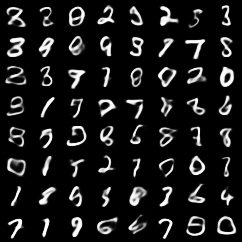
\includegraphics[scale=1]{Q3vaesample.png}
		\caption{Samples generated with VAE}
		\label{fig:q3vae}
	\end{figure}
	
	
	\begin{figure}[H]
		\centering
		\begin{subfigure}[b]{0.4\linewidth}
			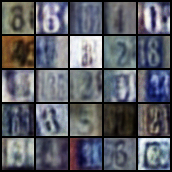
\includegraphics[scale=1]{Q3gansample.png}
		\end{subfigure}
		\begin{subfigure}[b]{0.4\linewidth}
			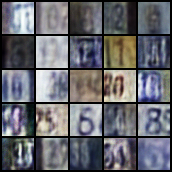
\includegraphics[scale=1]{Q3gansample2.png}
		\end{subfigure}
		\caption{Samples generated with GAN.}
		\label{fig:q3gan}
	\end{figure}

\item[2.]{Learning the disentangled representation in the latent space}
The following figures show how the GAN has learned a disentangled representation:
\begin{figure}[H]
	\centering
	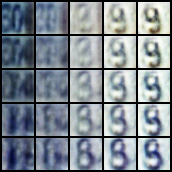
\includegraphics[scale=1]{gandesent1.png}
	\quad
	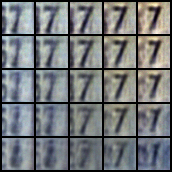
\includegraphics[scale=1]{gandesent2.png}
	\caption{Samples by perturbating the dimensions, left: 6 and 96, right: 25 and 75}
	\label{fig:des1}
\end{figure}

%\begin{figure}[H]
%	\centering
%	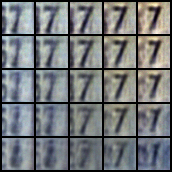
\includegraphics[scale=1]{gandesent2.png}
%	\caption{Samples by perturbating dimensions 25 and 75}
%	\label{fig:des2}
%\end{figure}

The following figures show how the GAN has learned a disentangled representation:
\begin{figure}[H]
	\centering
	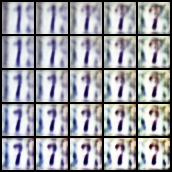
\includegraphics[scale=1]{sample_VAE21-65_epsilon_90.png}
	\quad
	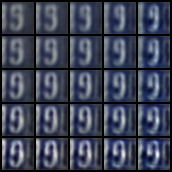
\includegraphics[scale=1]{sample_VAE21-8_epsilon_60.png}
	\caption{Samples by perturbating the dimensions, left: 65 and 90, right: 8 and 60}
	\label{fig:desVAE}
\end{figure}

\item[3.] {Interpolation in the data space and in the latent space:}

\begin{enumerate}
	\item VAE:\\
	Moving along $\alpha$, we observe a smooth transition from one sample to the other.
	
	\begin{figure}[H]
		\centering
		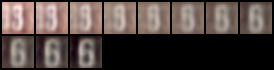
\includegraphics[scale=1]{vae_latent.png}
		\caption{Interpolation in the latent space using VAE}
		\label{fig:vae_latent}
	\end{figure}
	
	\begin{figure}[H]
		\centering
		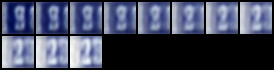
\includegraphics[scale=1]{vae_image.png}
		\caption{Interpolation in the data space using VAE}
		\label{fig:vae_image}
	\end{figure}

	\item GAN:\\ 
	\begin{figure}[H]
		\centering
		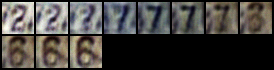
\includegraphics[scale=1]{GAN_latent.png}
		\caption{Interpolation in the latent space using GAN}
		\label{fig:gan_latent}
	\end{figure}
	
	\begin{figure}[H]
		\centering
		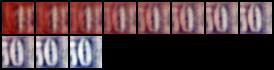
\includegraphics[scale=1]{GAN_image.png}
		\caption{Interpolation in the data space using GAN}
		\label{fig:gan_image}
	\end{figure}
	

	\end{enumerate}


\end{enumerate}

    \item [B.] {\textbf{Quantitative Evaluations}}\\
    \begin{enumerate}
        \item[1.] 
       We have used the provided functions to extract the representations of the images. We compute the Frechet Inception Distance by estimating the mean and covariance of the generator's/decoder's distribution. The calculation steps are explained in the following code snippet:
       \lstinputlisting[language=Python]{fid.py}
       
        \item[2.] We sampled 1000 images from each generative models and calculate the FID-score as instructed. The results are: 
        \begin{itemize}
        	\item For the GAN, the FID score is: $29 526.37$
        	\item For the VAE, the FID score is: $51 355.12$
        \end{itemize}
        This metric confirme our ascertainment that the GAN is more realistic than the VAE, given the ground truth given by the provided classifier.
        
    \end{enumerate}
\end{itemize}

